

\subsection{Scheduling CP}

\begin{center}
    \texttt{cumulative($[s_1,..., s_n], [d_1, ..., d_n], [e_1, ...,
    e_n], [c_1, ..., c_n], C$)}
\end{center}

\begin{itemize}
    \item $\forall_i: s_i + d_i = e_i$
    \item $\forall_t: \sum_{s_i \leq t < e_i} c_i \leq C$
\end{itemize}

\subsubsection{Sweep line algorithm}
It's use to compute the cumulated
profile and check that it does not exceed the capacity.


\begin{enumerate}
    \item \begin{tabular}{m{5cm}m{10cm}}
            \begin{itemize}
                \item One time point for start $(start, +capa)$
                \item One time point for end $(start, -capa)$ 
            \end{itemize}&
                    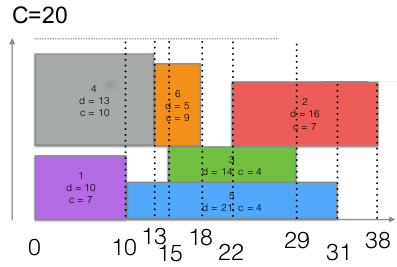
\includegraphics[width=7cm]{sweepLine}
                \end{tabular}


            \item \begin{tabular}{m{5cm}m{8cm}}
                    \begin{itemize}
                        \item Sort time points
                    \end{itemize}
                    &

                    (0,+7), (0,+10), (10,-7), (10,4), (13,-10), (13,9), (15,4), (18,-9), (22,7), (29,-4), (31,-4), (38,-7)
                \end{tabular}

            \item \begin{tabular}{m{5cm}m{10cm}}
                    \begin{itemize}
                        \item Sweep-line(t) = height of the profile at time $t$.
                    \end{itemize}
                    &
                    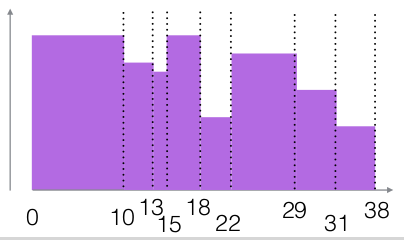
\includegraphics[width=7cm]{sweepLine2}
                \end{tabular}

                \begin{lstlisting}[mathescape]
input = eventQueue$[(time,c)]$
t = input.head.time   // Current time of the sweep line
h = 0                 //  current capacity of the sweep line 

while (input.nonEmpty) {
    while (input.nonEmpty && input.head.time == t){
        (time,c) = input.dequeue
        h = h + c
    }
    add (t,h) to the profile
    t = input.top.time
}
            \end{lstlisting}
    \end{enumerate}


\subsubsection{Optimistic Resource Profile}

\begin{tabular}{m{11cm}m{6cm}}
The optimistic resource profile is built based on the
\textbf{mandatory parts} which is the time where the activity will
use the resource whatever it final position.
&
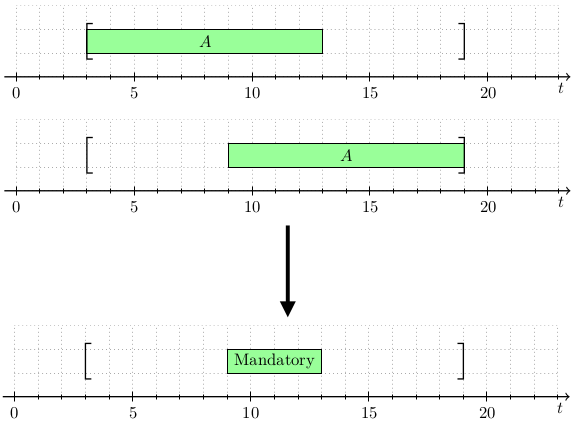
\includegraphics[width=4cm]{mandatory}
\end{tabular}

\begin{itemize}
    \item \textbf{Update minimum start time} at the earliest
        time such that it is not in conflict with the optimistic
        resource profile.

        \paragraph{Time complexity}: $O(n)$ per task since recource
        profile has $O(n)$ intervals. So, $O(n^2)$ overall.
\end{itemize}


\subsection{Large Neighborhood Search}

\begin{tabular}{m{12cm}m{3cm}}
    The diversification is the most weakness of CP for hard COPs.
    The idea of LNS is stuck for too long $\to$ jump in the search space
    by using restart!
    &
    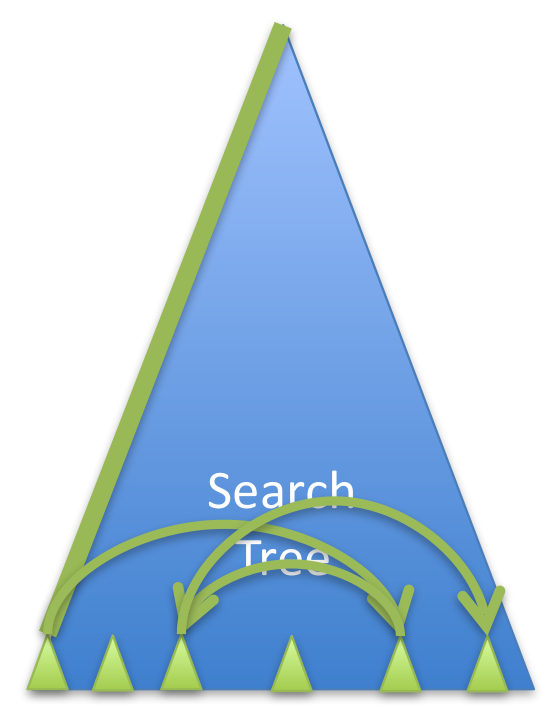
\includegraphics[width=2cm]{LNS}
\end{tabular}

\begin{tabular}{m{2cm}m{11cm}}
    Randomized restart & 
    \begin{itemize}
        \item Use some random decisions in your heuristic (value or variable)
        \item Use a limit on the search (number of backtracks or
            time)
        \item If no feasible solution is found within this limit,
            restart.
    \end{itemize}
\end{tabular}

\subsubsection{LNS work}

\begin{tabular}{m{10cm}m{6cm}}
    \begin{enumerate}

        \item Find a first initial solution, $S*$
        \item Randomly relax $S*$ and re-optimize with search limit

            Relax = fix some variables to their values in $S*$ and CP
            search the other

            \begin{itemize}
                \item A portion of the variables is selected (=\textbf{fragment})
                    and are relaxed to the \textbf{initial domain}
                \item The other variables are frozen to their value in the current solution
                \item A limited CP search \textbf{improving solutions}
            \end{itemize}

        \item Replace $S*$ by the best solution found
    \end{enumerate}

    &
    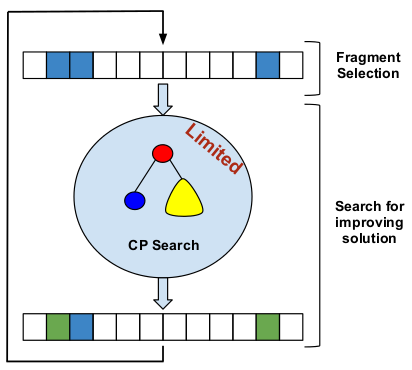
\includegraphics[width=6cm]{lns.png}
\end{tabular}

\paragraph{Advantages}
\begin{itemize}
    \item Good diversification if fragment well chosen $\Rightarrow$ no
        meta-heuristic needed (tabu,...) because neighborhood is large
        enough
    \item No need to design complex feasible neighborhoods because CP
        is in charge of feasibility

    \item Intensification with CP search and efficient 
        exploration of neighborhoods with CP
    \item Scalability of LS
\end{itemize}


\subsubsection{LNS parameters}
Parameters of LNS :
\begin{itemize}
    \item \textbf{Fragment size} and \textbf{time/backtrack limit}:
       strongly linked parameters because
       \begin{enumerate}
           \item fragment size determines neighborhood size
           \item limit determine the maximal effort to explore
       neighborhood.
       \end{enumerate}

       \paragraph{Note:} a good LNS should never be stopped only by the limit\ldots

       \paragraph{Adaptive versions}:
       \begin{enumerate}
           \item Fix a time/backtrack limit
           \item if neighborhood fully explored $\to$ increase fragment size
           \item else: decrease fragment size
       \end{enumerate}

    \item \textbf{fragment selection} (can be combined).

        Should contain important variables and related variables.

        \begin{itemize}
            \item \begin{tabular}{m{3cm}m{10cm}}
                    Random selection &
                \begin{itemize}
                    \item Surprisingly good
                    \item Generic
                    \item Excellent diversification
                    \item Intensification from CP search
                \end{itemize}
            \end{tabular}

        \item \begin{tabular}{m{3cm}m{10cm}}
                    Specific selection &
                \begin{itemize}
                    \item Only for one problem
                    \item Use knowkedge of the problem to select variables
                    \item Usually randomized to some extend
                \end{itemize}
            \end{tabular}
        \end{itemize}
\end{itemize}

\subsubsection{QAQ}
\begin{tabular}{m{9cm}m{7cm}}
    \begin{lstlisting}
val	cp	=	CPSolver()	
var	w:	Array[Array[Int]]		//weight	matrix	
var	d:	Array[Array[Int]]		//distance	matrix	
val	x	=	N	map	(v	=>	CPIntVar(cp,	0	until	n))	
//matrix	of	variables			representing	the	distances	
val	D	=	Array.tabulate(n,	n)((i,	j)	=>		
									element(d,	x(i),	x(j)))	
val	bestSol	=	Array.fill(n)(0)	
cp.onSolution	{	
	for(i	<-	0	until	n)		
			bestSol(i)	=	x(i).value)	
}	

add(allDifferent(x),	Strong)
minimize(sum(N,	N)((i,	j)	=>	D(i)(j)	*	w(i)(j)))	
search	{	
		binaryFirstFail(x)	
}	start(1)
\end{lstlisting}
&
\begin{lstlisting}[caption=LNS relax]
for (r <- 1 to 300) {
    startSubjectTo(failureLimit = 60) {
        // relax randomly 50% of the variables
        for (i <-N; if rand.nextInt(100) < 50) {
            add(x(i) == bestSol(i))
        }
    }
}
\end{lstlisting}

\begin{center}
    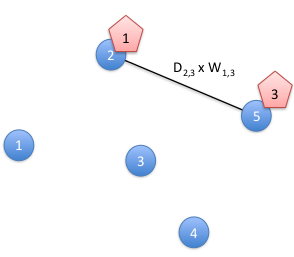
\includegraphics[width=4cm]{QAP}
\end{center}
\end{tabular}

\subsubsection{Vehicle routing}

\textbf{Regret heuristics}: choose the variable with the
greatest difference in cost between the two best values in
its domain. i.e. Measure the impact of not having the best
choice.

\begin{itemize}
    \item Remove the longest arcs in order to have a chance to improve
    \item From routes that are close such that you can relocate customers
\end{itemize}

\subsubsection{Cutting stock}

    \begin{itemize}
        \item $X_i \in N$: the number of planks with configuration $i$
            produced where a configuration is a possible assignment of
            roll type to a plank.

        \item Configuration $i: [a_{1i}, a_{2i}, ..., a_{ni}]$ where
            $a_{ji}$ is the number of roll type $j$ (width $w_j$) in
            configuration $i$.

            Note that there is a exponential number of
            configurations
    \end{itemize}

\begin{tabular}{m{5cm}cm{5cm}}
    \begin{eqnarray*}
        \textrm{minimize } & \sum_i X_i \\
        \textrm{Subject to } & \sum_i X_i a_{ji} \geq b_j
        \forall_j\\
        & x_i \geq 0
    \end{eqnarray*}
    & $\Leftrightarrow$ Strong LP duality $\Leftrightarrow$ & 
    \begin{eqnarray*}
        \textrm{minimize } & \sum_i b_i Y_i \\
        \textrm{Subject to } & \sum_i Y_i a_{ji} \geq 1
        \forall_j \\
        & Y_i \geq 0
    \end{eqnarray*}
\end{tabular}

\begin{center}
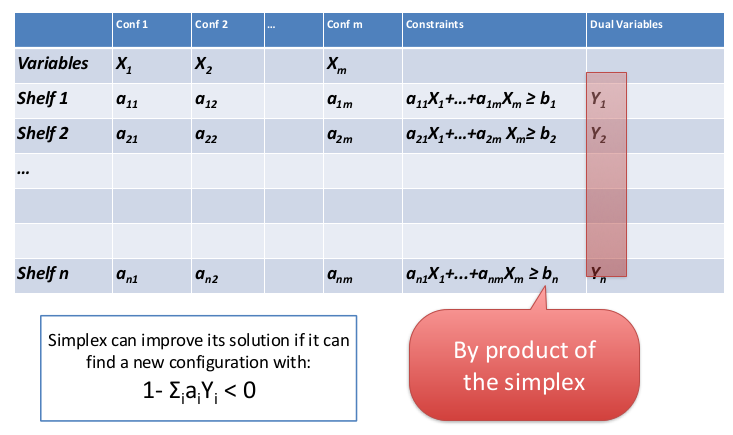
\includegraphics[width=13cm]{column}
\end{center}

\begin{itemize}
    \item Find a configuration $[\alpha_1, ..., \alpha_n]$ such that:
        $$1 - \sum_i \alpha_i Y_i < 0$$
        If there isn't such configuration, we prove the optimality of the
        linear program

    \item[$\Rightarrow$] Pricing is a Knapsack problem:
        \begin{eqnarray*}
            \textrm{Maximize } & \sum_i \alpha_i Y_i\\
            \textrm{Such that } & \sum_i \alpha_i w_i \leq W
        \end{eqnarray*}

        Note that $\alpha_i$ are the variables and $Y_i$ are constants
        given as by product of the simplex
\end{itemize}

\begin{center}
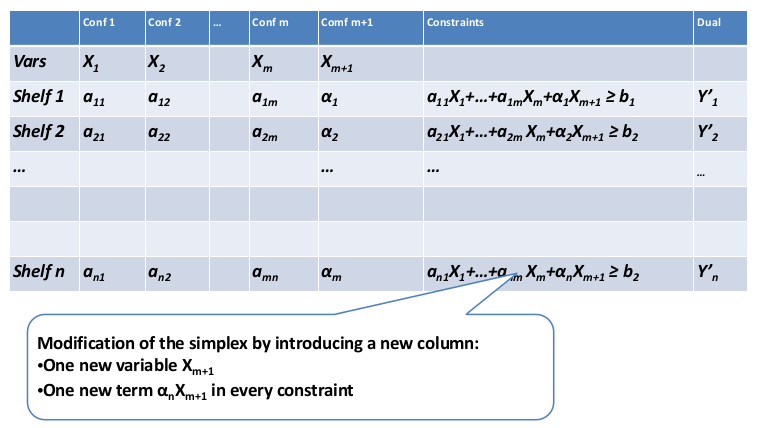
\includegraphics[width=13cm]{column2}
\end{center}


\paragraph{Column generation}
\begin{enumerate}
    \item Start with a limited number of patterns
    \item Solve the master problem 
    \item  Generate a new column (with CP/LS/B\&B/...) with negative reduced cost, if
        not possible stop
\end{enumerate}

\paragraph{Column generation by SINFO22}
\begin{enumerate}
    \item Generate a few valid columns to start with

    \item  Solve the dual problem using simplex to get optimal $Y_i$ directly,
        or solve the primal problem to get optimal $X_i$ which you can then
        use to compute the optimal $Y_i$ using complementarity conditions.
        Both these techniques were not seen in class, although if you know
        the dual problem, applying simplex on it is just as easy as applying
        it on the primal.

    \item  Once you have the $Y_i$, you need to find 'a' such that $1 - \sum_i
        Y_i * a_i$ is negative. If you find such an $a$, you can include as a
        new pattern in your simplex tableau and since the reduced cost is
        negative, it will help reduce the objective. You could use any 'a'
        that produces negative reduced cost, but it's better to pick the
        most negative one directly. Since minimizing $1-\sum_i Y_i*a_i$ is
        equivalent to maximising $\sum_i Y_i * a_i$, you will solve the
        maximization problem instead. You cannot pick any 'a' because it
        still need to be a valid pattern (it must fit on a plank...), so you
        have to add the $\sum_i a_i <= L$ constraint where L is the length of
        the plank.

    \item  Now you have a new pattern, and you can include it in your
        simplex. You then iterate your simplex until you find an optimal
        solutions that uses only the few columns that you included. When you
        reach the optimum, you don't know if it's the real optimum of the
        problem because you're only looking at solutions using a few
        columns. You need to restart at step 3 and keep adding columns until
        step 3 can't find a column with negative reduced cost (the
        maximization procedure will give a value <= 1. When that's the case,
        you know you're done).
\end{enumerate}

\paragraph{Hybridization}

Is it because, on one hand, we have a linear program for minimizing an
objective with a limited set of column, and on the other hand, we have
another algorithm (e.g. Branch \& Bound, Local search, LNS,...) for
generating a column with the smallest negative reduced cost (if such a
column exists) ?
So we have an hybridization between the linear program and the other
algo ?


\subsection{Exam}
\begin{itemize}
    \item  Be able to explain the sweep line algorithm and be
        able to execute it to compute a resource profile
    \item  Understand how to use the (optimistic) resource profile
        to filter the domain of start/end variables
    \item  Explain what is LNS, what is the advantage of using it
        over pure CP, what do we loose (proof of optimality)?
    \item  Be able to suggest LNS relaxation for a problem
    \item  Explain what is column generation. In what sense does
        it allow hybridization
\end{itemize}



